\documentclass[10pt]{standalone}
\input{../../tikzpic_packages.tex}

\begin{document}
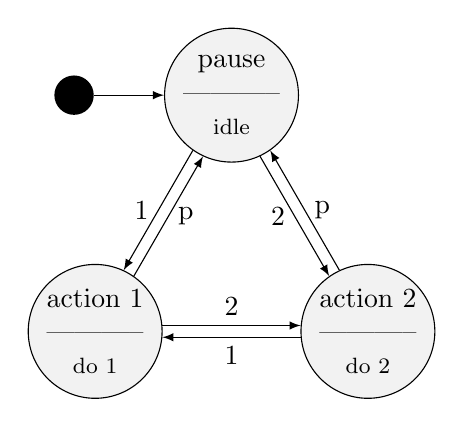
\begin{tikzpicture}[
scale = 2,
state/.style={draw, circle, fill=gray!10, minimum width=1.7cm, align=center, inner sep= 0pt},
trans/.style={-latex},
initialstate/.style={circle, fill, minimum width=.5cm, inner sep=0pt}
]

\path (90:1)node[state](p){pause \\ ----------- \\ \footnotesize{idle}};
\path (210:1)node[state](1){action 1\\ ----------- \\ \footnotesize{do 1}};
\path (330:1)node[state](2){action 2\\ ----------- \\ \footnotesize{do 2}};
\path (p)++(-1,0)node[initialstate](i){};

\draw[trans] (i)--(p);

\draw[trans] (p.235)--(1.65)node[midway, left]{1};
\draw[trans] (1.55)--(p.245)node[midway, right]{p};

\draw[trans] (p.-65)--(2.125)node[midway, left]{2};
\draw[trans] (2.115)--(p.-55)node[midway, right]{p};

\draw[trans] (1.5)--(2.175)node[midway, above]{2};
\draw[trans] (2.185)--(1.-5)node[midway, below]{1};


\end{tikzpicture}
\end{document}